\usepackage{tikz}
\usetikzlibrary{shapes.geometric, arrows}

\tikzstyle{process} = [rectangle, minimum width=3.0cm, minimum height=1.5cm, text centered, draw=black]
\tikzstyle{arrow} = [thick,->,>=stealth]

\begin{figure}
\centering
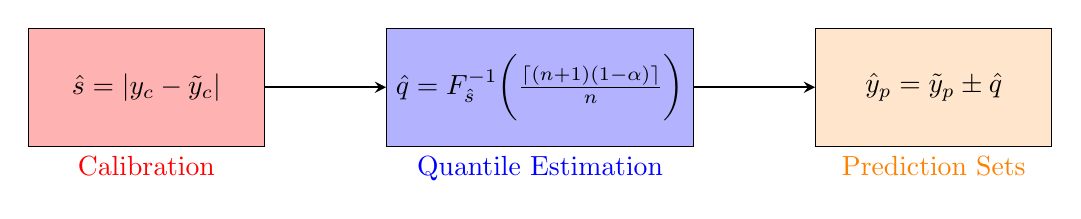
\begin{tikzpicture}[remember picture, node distance=5.0cm]
    \node (start) [process, fill=red!30, label={[font=\color{red}]below:Calibration}] {$\hat{s} = |y_c - \tilde{y}_c|$};
    \node (step) [process, fill=blue!30, label={[font=\color{blue}]below:Quantile Estimation}, right of=start] {$\hat{q} = F^{-1}_{\hat{s}}\bigg(\frac{\lceil(n+1)(1-\alpha)\rceil}{n}\bigg)$};
    \node (end) [process, fill=orange!20, label={[font=\color{orange}]below:Prediction Sets}, right of=step] {$\hat{y}_p = \tilde{y}_{p} \pm \hat{q}$};

    \draw [arrow] (start) -- (step);
    \draw [arrow] (step) -- (end);
\end{tikzpicture}
\caption{Inductive CP framework using Absolute Error Residual (AER) nonconformity scores (see \cref{nonconformity scores}): (1) Calibrate by computing nonconformity scores ($\hat{s}$) from calibration predictions ($\tilde{y}_c$) and targets ($y_c$). (2) Estimate the quantile ($\hat{q}$) for desired coverage $(1-\alpha)$ using $n$ calibration samples and the inverse CDF $F_{\hat{s}}^{-1}$. (3) Construct prediction sets by applying $\hat{q}$ to test predictions ($\tilde{y}_p$).}
\label{fig: cp_framework_tikz}
\end{figure}
    